\subsection{The (Discrete) Fourier Transform}
The classical tool for analyzing oscillations is the Fourier Transform. One of the major problems of using this tool is the fact that 
it is only possible to look at the spectra of the oscillations (and so, how the amplitudes of the oscillations are distributed in the frequency domain). 
To introduce how transient and aperiodic signals are represented in the spectral domain, the Dirac delta can be used, whereby a single non-zero value 
in the time domain is represented by constant power across all frequencies in the frequency domain (\textit{Figure (a)}). This illustrates that power in a specific 
frequency band does not generally correspond to a present oscillation in the time domain.\\
Similarly, \(1/f\)-like aperiodic activity (\textit{pink noise}), which is common in neural data, shows power across all frequencies, with decreasing power for 
higher frequencies (\textit{Figure (b)}). 
Despite the lack of periodic activity in aperiodic time series, narrowband filtering, which imposes a sinusoidal basis, extracts components that appear to be oscillatory, 
when filtered into canonical band ranges (\textit{Figure (c)}).\\
There is another aspect that is crucial: using the periodogram (either the standard or the modified Welch), what usually is done is to separate the signal in different time-windows of 
a given length, to perform the \textit{fft}, for each window and then to average all of them. The time-window length is defined at the beginning of the algorithm, and then it runs across 
all possible windows. If there is a signal that is constant in energy across time (such as a sinusoid), it's not important the duration of the window; if the signal is very different from 
a sinusoid (that is the case of neuronal oscillations), the selectioned window acts as a low-pass filter: for this reason, there is not an optimal way to select the window length. Ideally, 
the best way is to have a time-window that is dependent on the frequency taken into account, but this is not possible in the Fourier Analyses.
\begin{figure}[H]
    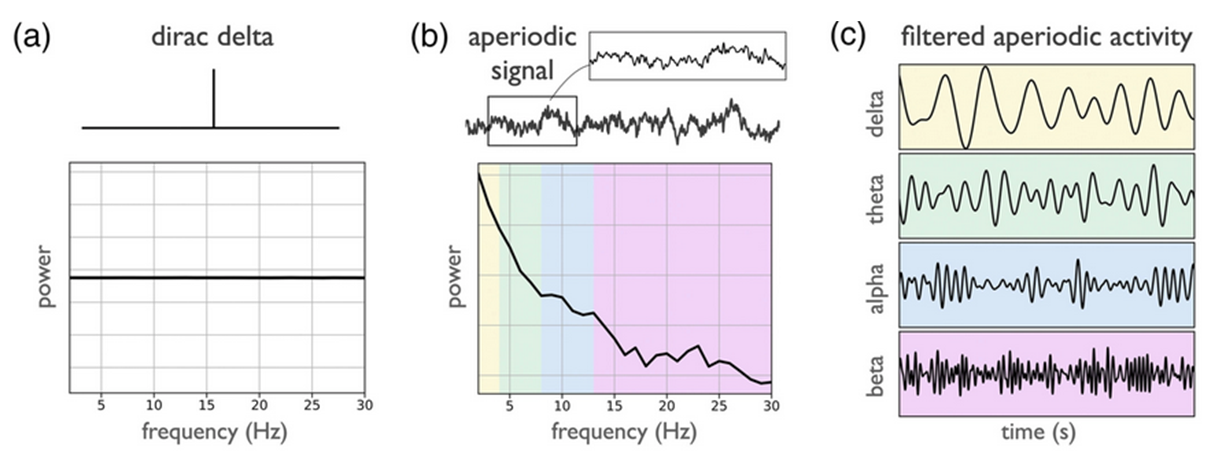
\includegraphics[scale=0.40]{11_1}
    \centering
\end{figure}
What can be done is to concentrate the analysis in the so called \textbf{frequency peaks}. In general, the procedure is to take the spectrum, 
to localize the point in frequency (or the frequency range) where there is the maximum amplitude, because large increases have probably some sort of oscillations. 
Then the analysis can be focused on that specific region of the frequency spectrum.\\
Neural oscillations display significant variations in their peak frequencies, including variation across age, within and between participants, 
and across cortical locations. Alpha peak frequency, for example, is considered a stable trait marker, and is also associated with some clinical disorders, displaying, 
for example, a slower frequency in attention-deficit hyperactivity disorder (ADHD). 
\par\medskip 
Due to frequency variation, even if the presence of oscillations is verified, the use of canonically defined frequency ranges may still fail to accurately reflect the 
data, as this may misestimate power of an oscillation if the spectral peak is not well captured in the canonical range. For example, a canonically defined alpha range 
of \(8-12\,Hz\) captures the peak of a \(10\,Hz\) oscillation (\textit{Figure (a)}), but fails to accurately capture an \(8\,Hz\) peak (\textit{Figure (b)}).
\begin{figure}[H]
    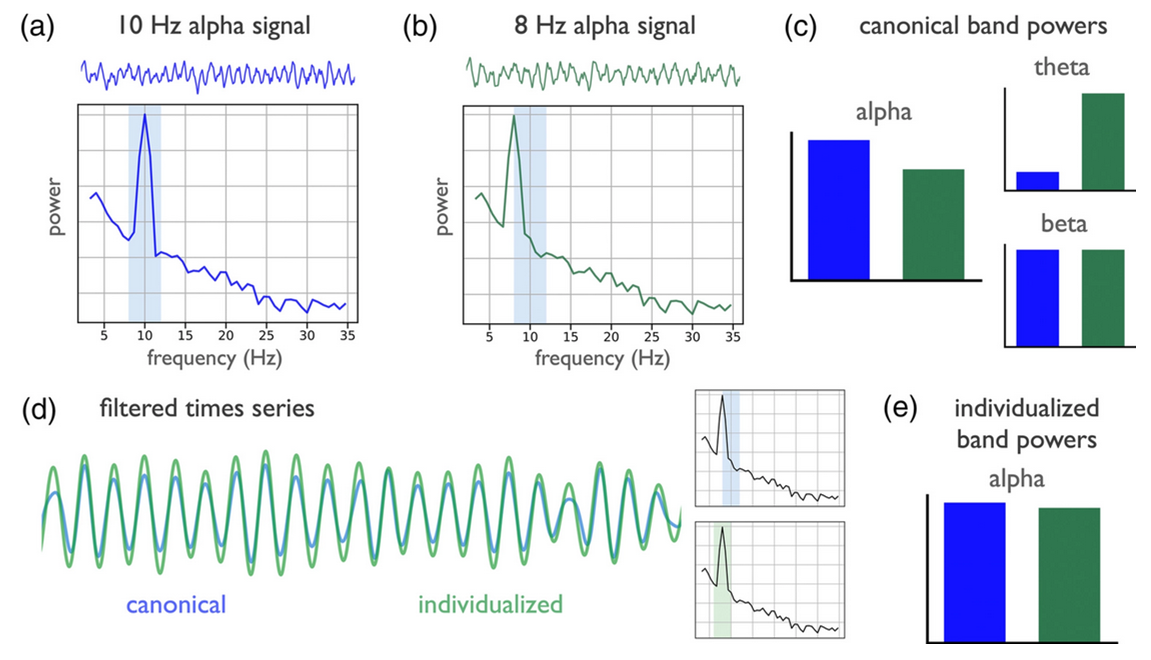
\includegraphics[scale=0.35]{11_2}
    \centering
\end{figure}
The Fourier Transform decomposes the signal in a weighted sum of complex sinusoids:
\begin{equation*}
    X_k=\sum_{n=0}^{N-1} x_n\cdot e^{-\frac{i2\pi}{N}\cdot kn}
\end{equation*}
What does it happen if the signal is significantly non-sinusoidal? The neuronal oscillations are highly non-stationary. In this way, Fourier Transform may not 
be the best way to look at the activity. Another possibility to characterize the properties is to look at the spectrum, to define the frequency band of interest, to filter 
the activity there, and then go back to the time domain and quantify what is the distance that the oscillation has from the sinusoid. One possibility is to create a \textit{time-resolved 
peak-through symmetry} (or asymmetry), understanding how much these peak-through distances are different from a pure sine.

\subsubsection{Periodic and Aperiodic Components}
The Power Spectrum of a brain signal is usually distributed following a \textit{Power-Law Distribution}, that decays as the frequency increases at the power of an \(alpha\) parameter, 
that controls the slope of the decay.\\
There are a lot of evidences that suggest that the decay depends on several physiological or patological parameters: for this reason, it is not considered as noise.
\par\medskip
One of the first thing to do in a Fourier-based analysis is to separate the periodic (the brain oscillations) from the aperiodic spectral components. One possibility is to use the algorithm 
of \textit{Donoghue T. et al., 2020}, which can be explained in the following steps:
\begin{figure}[H]
    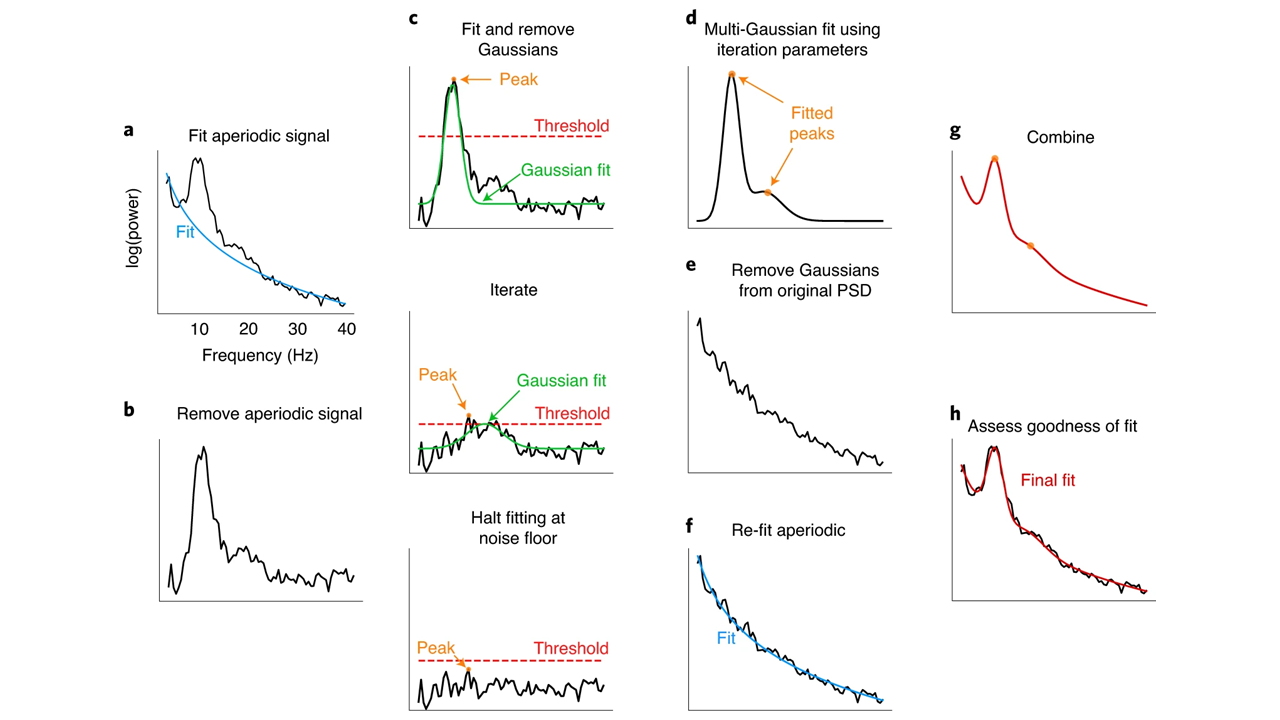
\includegraphics[scale=0.30]{11_3}
    \centering
\end{figure}
\begin{itemize}
    \item[\textbf{a)}] The PSD is first fit with an estimated aperiodic component (blue);
    \item[\textbf{b)}] The estimated aperiodic portion of the signal is subtracted from the raw PSD, the residuals of which are assumed to be a mix of periodic oscillatory peaks and noise;
    \item[\textbf{c)}] The maximum (peak) of the residuals is found (orange). If this peak is above the noise threshold (dashed red line), calculated from the standard deviation of the residuals, 
    then a Gaussian (solid green line) is fit around this peak based on the peak's frequency, power and estimated bandwidth. The fitted Gaussian is then subtracted, and the process 
    is iterated until the next identified point falls below a noise threshold or the maximum number of peaks is reached;
    \item[\textbf{d)}] Multi-Gaussian fitting is then performed on the aperiodic-adjusted signal from \textbf{b} to account for the joint power contributed by all of the putative oscillations together;
    \item[\textbf{e)}] This multi-Gaussian model is then subtracted from the original PSD from \textbf{a};
    \item[\textbf{f)}] A new fit for the aperiodic component is estimated;
    \item[\textbf{g)}] This re-fit aperiodic component is combined with the multi-Gaussian model to give the final fit;
    \item[\textbf{h)}] The final fit (red).
\end{itemize}
\par\medskip
Another method to separate the aperiodic component from the periodic one is the \textbf{Irregular-Resampling Auto-Spectral Analysis (IRASA)}. This algorithm starts from the idea 
that noise is a scale-free property of the system, while the brain oscillations are strongly dependent on the time interval of interest. IRASA resamples the time course of the activity 
at different scales (both downsampling and upsampling), and it repeats the Fourier analysis at every different resampling factor. When there is a resampling, the peak of the oscillations 
move, depending on the kind of resampling. Doing this for multiple times and taking the median of all possible resamplings, what remains is just the scale-free component, and so the aperiodic 
component.
\begin{figure}[H]
    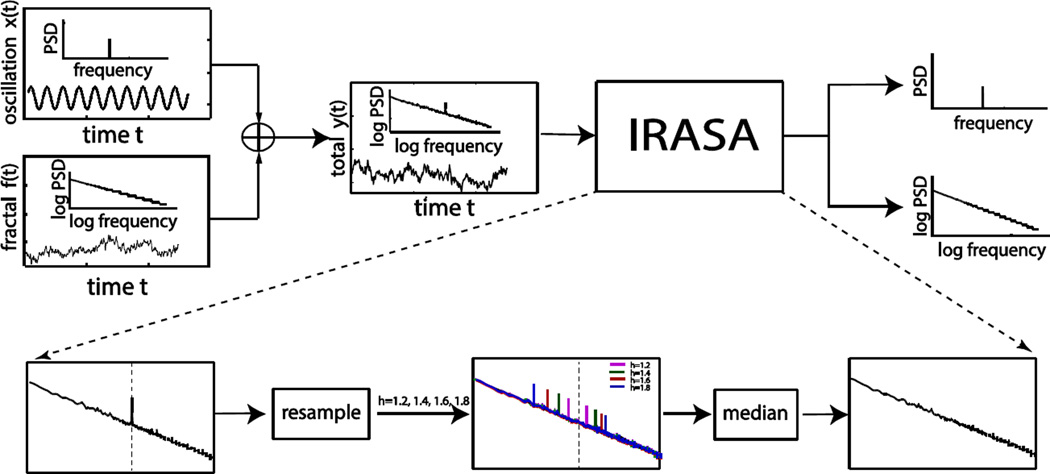
\includegraphics[scale=0.40]{11_4}
    \centering
\end{figure}
Of course, these two systems have some drawbacks: for the first one, if the initial fit is not appropriate, then the overall analysis will be strongly affected. If the decay changes its shape at 
some point, from a pure power-law to the noise level of the amplifier, the initial fit will be affected from the plateau, distrupting all the initial fitting.\\
For the second method, it is foundamental to correctly select the resampling factor when there are multiple peaks of different sizes, because the broad peak requires a larger sampling factor, while 
a smaller peak requires a smaller resamplig factor; if this is not done, the activity will be not completely separated.
\begin{itemize}
\item In the study of \textit{Voytek B. et al, 2020} was found that the aperiodic exponent is linked to brain maturation: when the brain evolves from the early childhood 
to adulthood, the aperiodic exponent usually becomes less steep. Also in the first days of life this behavior can be noticed:
\begin{figure}[H]
    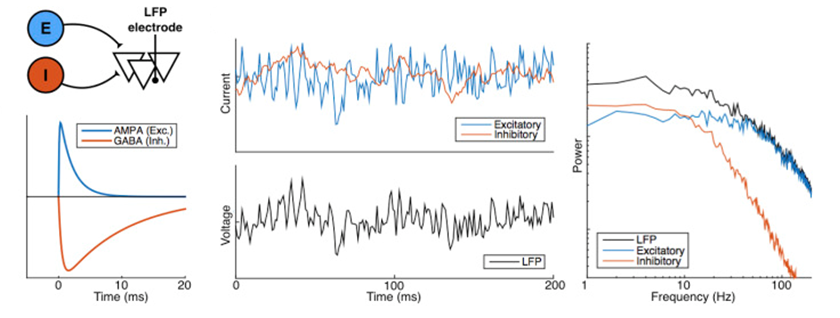
\includegraphics[scale=0.35]{11_5}
    \centering
\end{figure}
\par\medskip
\item It was found that the aperiodic exponent is also correlated with the excitation/inhibition (\(E/I\)) balance. In a study of 2017, Richard Gao created a small model 
of excitatory and inhibitory populations (that both simulated the action of pyramidal neurons). Looking separately at the excitatory and inhibitory components in 
the PSD, it is evident that the inhibitory component has a faster decay with respect to the excitatory one: in that sense, the aperiodic component can be used as a possible 
correlation with a larger inhibitory activity.
\begin{figure}[H]
    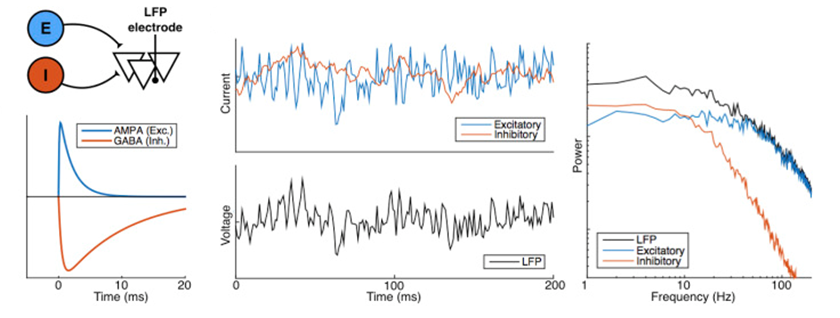
\includegraphics[scale=0.40]{11_6}
    \centering
\end{figure}
\end{itemize}

\paragraph{PSDs Limitations}
\begin{itemize}
    \item Brain oscillatory signals violate stationary requirement of Fourier-based analysis.
    \item Fourier-based spectral decomposition can tell whether an oscillation is present but not when (or where) it occurs.
\end{itemize}

\subsection{Short Time Fourier Transform}
The \textit{Short Time Fourier Transform (STFT)} is another possibility to access the time-frequency decomposition.
It consists in performing the Fourier Transform in smaller time-windows of a given length, and then look at them as a 
2-dimensional plot. Instead of separating the signal in multiple time-windows and then average across them, the window 
dimension is kept and all the Fourier Transforms are aligned into time bins. The larger the time bin, the better the 
frequency resolution but the worse the temporal resolution (for the \textit{Heisenberg Uncertainty Principle}).
\par\medskip
The problem of this method is that it's still Fourier-based. What can be done is to repeat the procedure for more than one 
time-window, adding another dimension. This will increase the total computational cost and the full analysis will be very 
complicated.

\paragraph{Fourier Analysis Limitations}
\begin{itemize}
    \item Fourier doesn't provide temporal information on discrete increase of amplitude of an oscillation (sine is always the 
    same across time).
    \item Fixed widths of time-windows in STFT creates a problem in neuroscience (because signals need to be stationary to be 
    able to apply the Fourier theorem).
\end{itemize}

\subsection{Wavelet Transform}